\documentclass[twocolumn]{article}

\usepackage{graphicx}
\usepackage{listings}
\usepackage{lmodern}
\usepackage{booktabs}
\usepackage{amsmath}
\usepackage{amssymb}
\usepackage{amsthm}
\usepackage{bbm}
\usepackage{multirow}
\usepackage{booktabs}
\usepackage{cancel}
\usepackage{hyperref}


%Math commands
\newcommand{\ev}[1]{\mathbb{E}\left(#1\right)}
\newcommand{\ov}[1]{\mathbb{O}(#1)}
\newcommand{\rmd}{\mathrm{d}}
\newcommand{\intg}[4]{\int_{#1}^{#2} \! #3 \, \rmd#4}
\newcommand{\der}[2]{\frac{\rmd^#1}{\rmd #2^#1}}


%Sectioning commands
\newcommand{\setsection}[1]{\setcounter{section}{#1}\addtocounter{section}{-1}\section{}}
\renewcommand{\thesubsection}{\alph{subsection})}
\renewcommand{\thesubsubsection}{
	\alph{subsection}.
	\arabic{subsubsection}
}

%Listings commands
\newcommand{\includecode}[1]{\lstinputlisting{#1}}
\newcommand{\code}[1]{\lstinline{#1}}

%Common settings
\lstset{language=R,basicstyle=\ttfamily}
\graphicspath{ {./img/} }
\author{Nakul Joshi}

\newcommand{\img}[1]{
\begin{figure}[!ht]
\centering
\includegraphics[width=0.4\textwidth]{#1}
\end{figure}
}

\newcommand{\N}[2]{\sim\mathcal{N}\left(#1,#2\right)}

\title{Math 308 Assignment 4\\Exercises 2.8}
\author{Nakul Joshi}

\begin{document}
\maketitle

\setsection{2}
$
\overline{x}=6.5\\
m=5.5\\
\tilde{x}=2.389726\\
\tilde{m}=2.342779\\
f(\overline{x})\neq \tilde{x}\\
f(m)\neq \tilde{m}
$

\setsection{4}

\subsection{}
\begin{table}[h]
\centering
    \begin{tabular}{ccccc}
    4-8am & 8-Noon & Noon-4pm & 4-8pm & 8-Mid \\
    699   & 1053   & 1048     & 972   & 257   \\
    \end{tabular}
\end{table}
\begin{figure}[h]
\centering
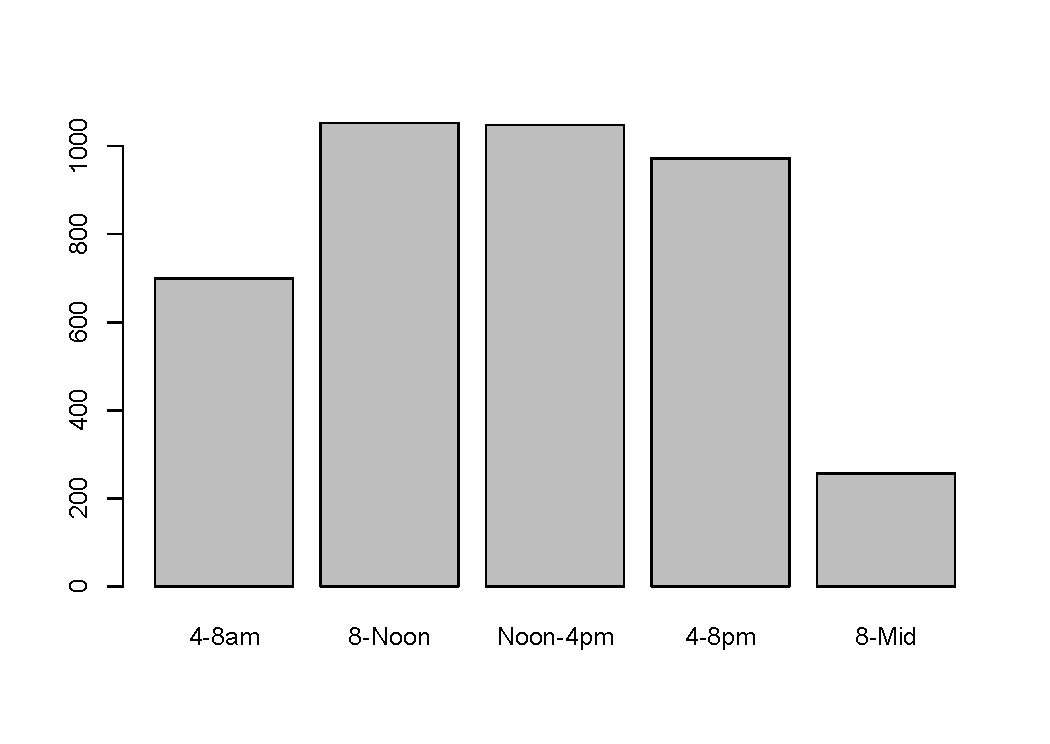
\includegraphics[width=0.4\textwidth]{4a.pdf}
\end{figure}

\newpage

\subsection{}
\vspace{-3em}
\begin{table}[h]
\centering
\begin{tabular}{@{}lrrr@{}}
\toprule
  & No  & Yes & Proportion \\ \midrule
Mon & 569 & 61  & 0.09682540 \\
Tue & 535 & 93  & 0.14808917 \\
Wed & 488 & 76  & 0.13475177 \\
Thu & 434 & 132 & 0.23321555 \\
Fri & 493 & 144 & 0.22605965 \\
Sat & 406 & 47  & 0.10375276 \\
Sun & 507 & 44  & 0.07985481\\
\bottomrule
\end{tabular}
\end{table}

\subsection{}
\vspace{-7pt}
\begin{figure}[!ht]
\centering
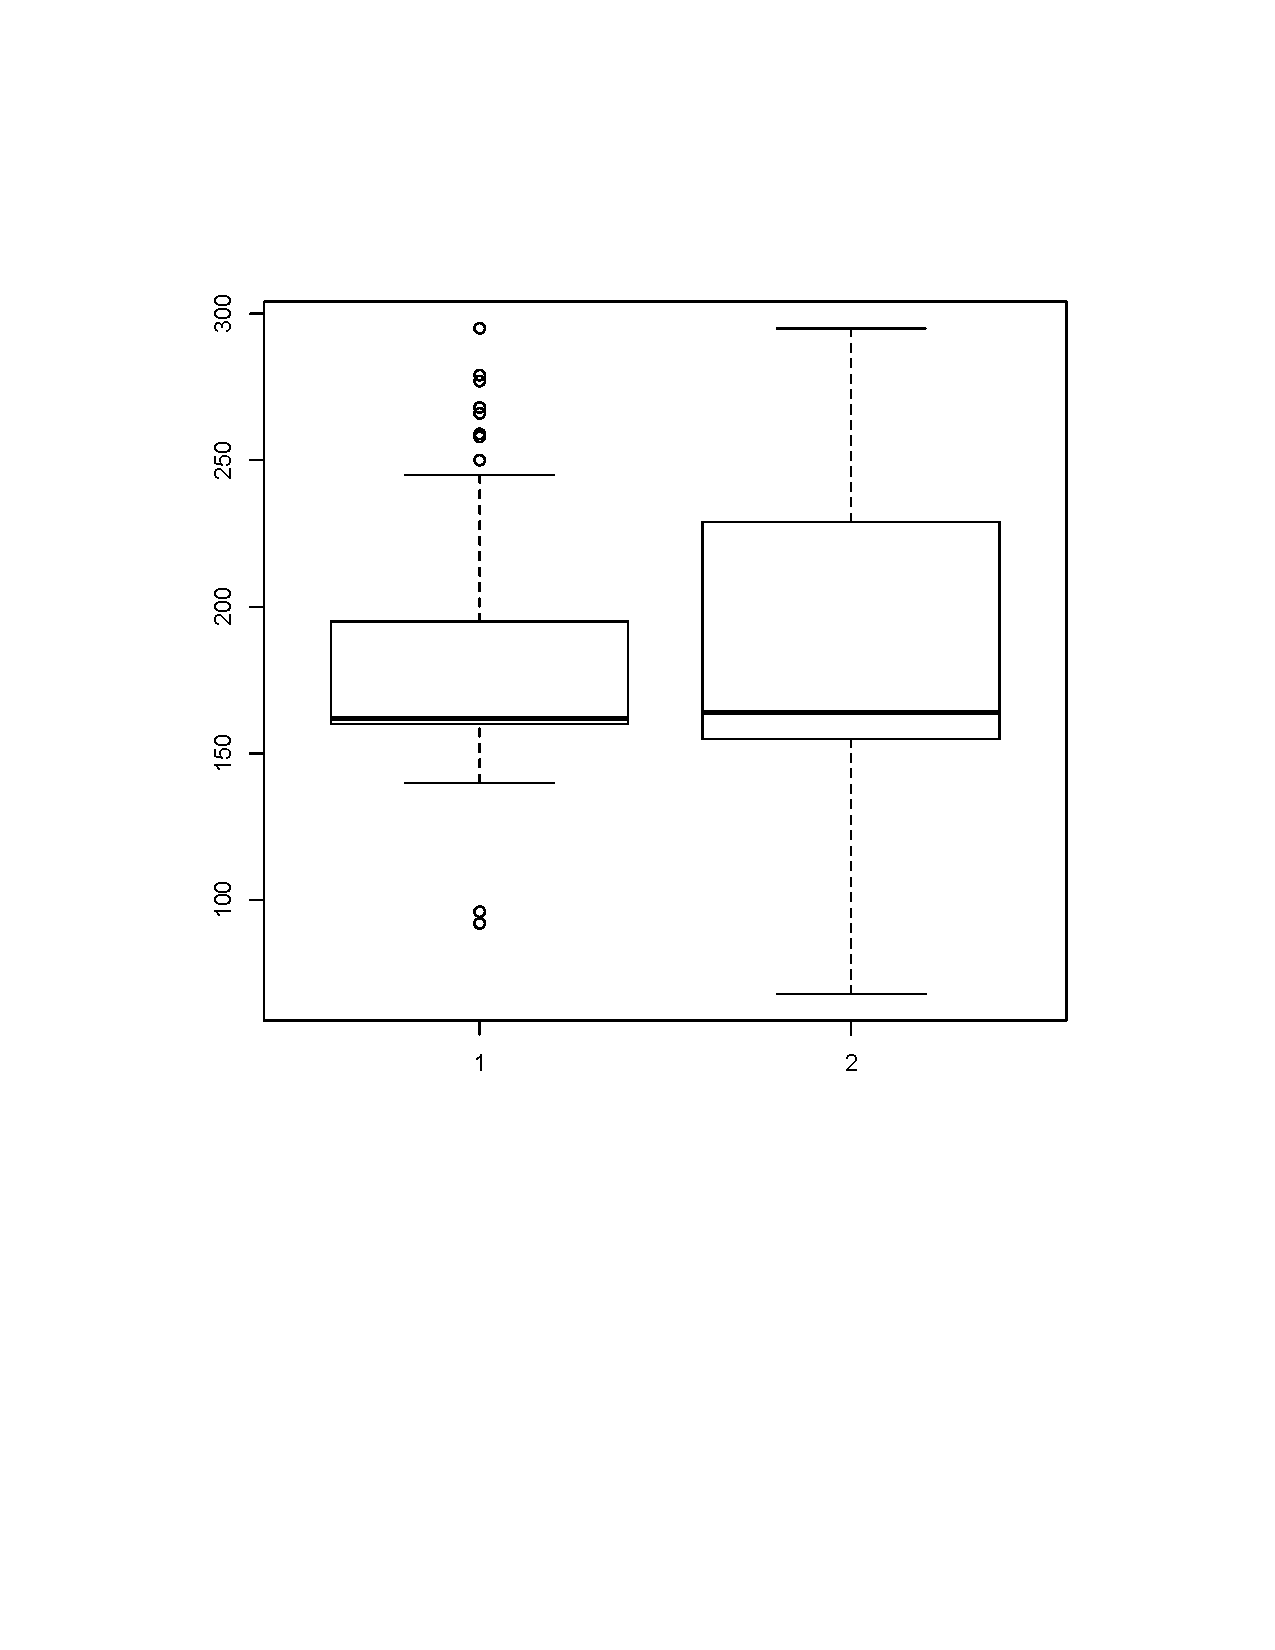
\includegraphics[width=0.4\textwidth]{4c.pdf}
\end{figure}


\subsection{}
There appears to be no relationship.

\setsection{6}

\subsection{}
\vspace{-1em}
\begin{table}[h]
\centering
\begin{tabular}{@{}llllll@{}}
\toprule
Min. & 1st Qu. & Median & Mean  & 3rd Qu. & Max.  \\ \midrule
8.30 & 23.20   & 30.10  & 30.93 & 38.17   & 51.50  \\ \bottomrule
\end{tabular}
\end{table}

\subsection{}
\begin{figure}[!ht]
\centering
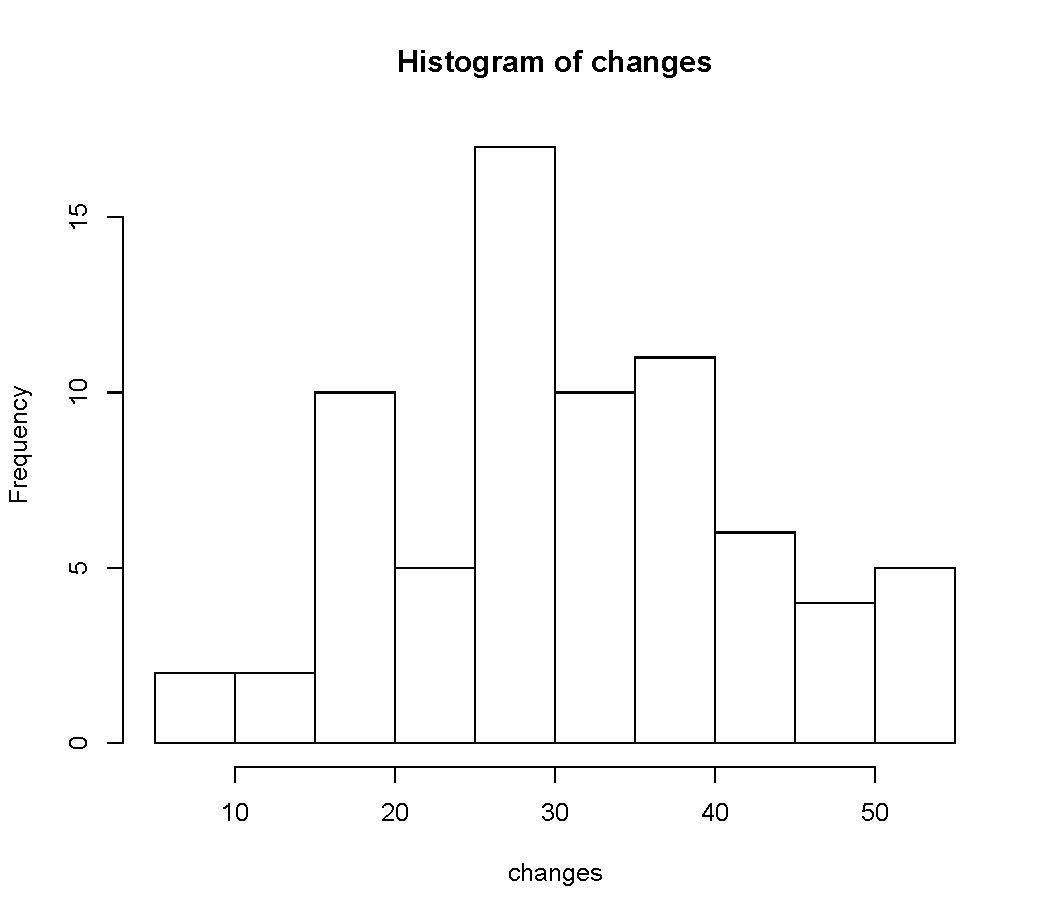
\includegraphics[width=0.4\textwidth]{6b1.pdf}
\end{figure}
\begin{figure}[!ht]
\centering
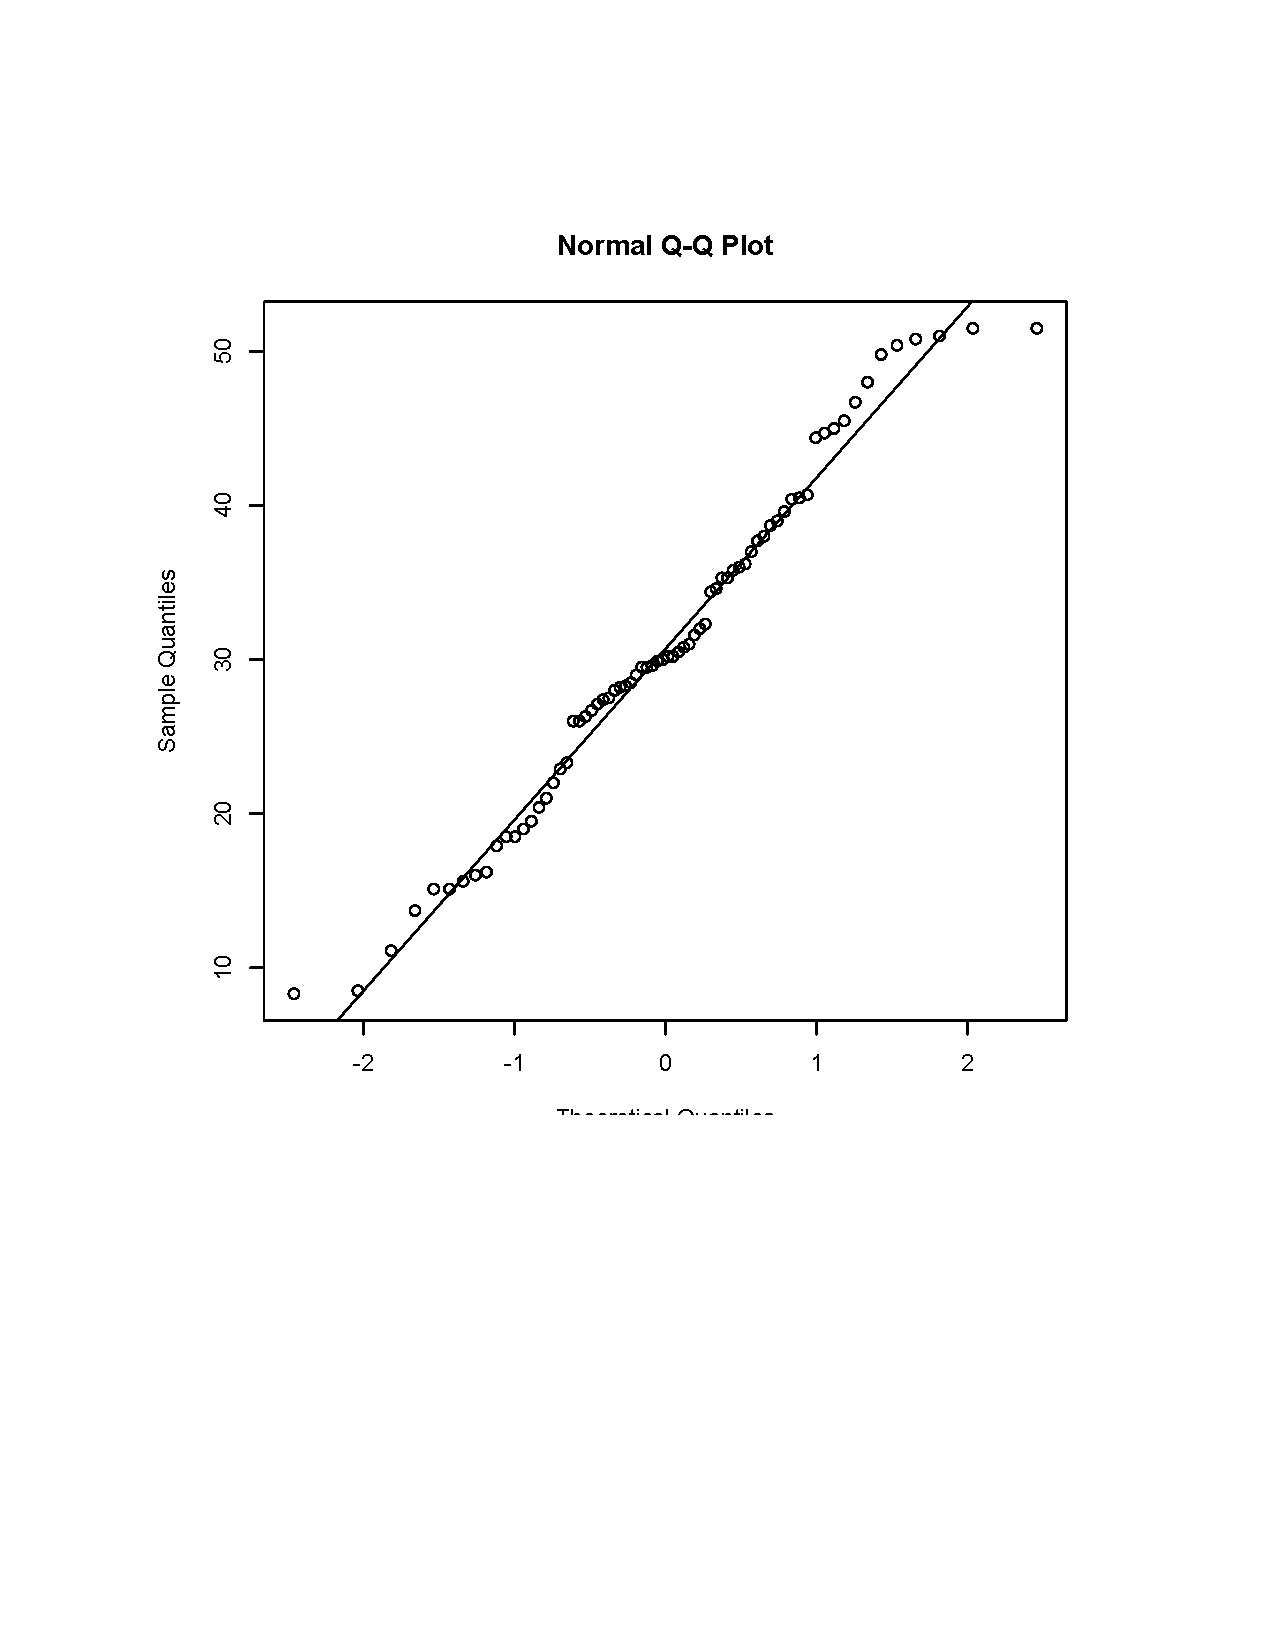
\includegraphics[width=0.4\textwidth]{6b2.pdf}
\end{figure}

The distribution is approximately normal as shown by the close fit between the normal and theoretical quantiles.

\subsection{}
\begin{figure}[h]
\centering
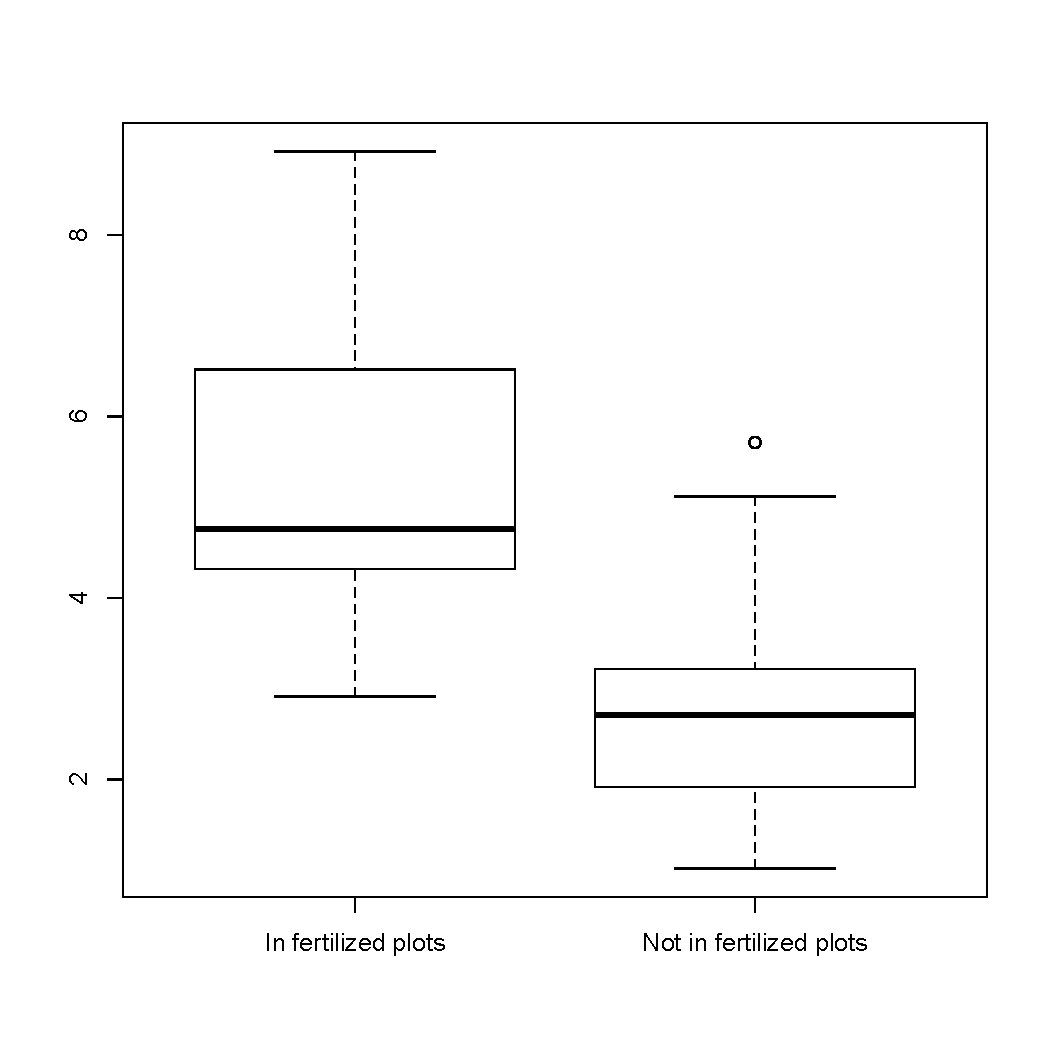
\includegraphics[width=0.4\textwidth]{6c.pdf}
\end{figure}

\subsection{}
% Booktabs require to add \usepackage{booktabs} to your document preamble
\begin{table}[h]
\begin{tabular}{@{}llllll@{}}
\toprule
Min.  & 1st Qu. & Median & Mean  & 3rd Qu. & Max.  \\ \midrule
2.912 & 4.318   & 4.762  & 5.274 & 6.518   & 8.919 \\ \bottomrule
\end{tabular}
\caption{Summary of F}
\end{table}
\begin{table}[h]
\begin{tabular}{llllll}
\toprule
Min.  & 1st Qu. & Median & Mean  & 3rd Qu. & Max.  \\ \midrule
1.019 & 1.915   & 2.712  & 2.718 & 3.165   & 5.712 \\ \bottomrule
\end{tabular}
\caption{Summary of NF}
\end{table}

\newpage

\subsection{}
\begin{figure}[h]
\centering
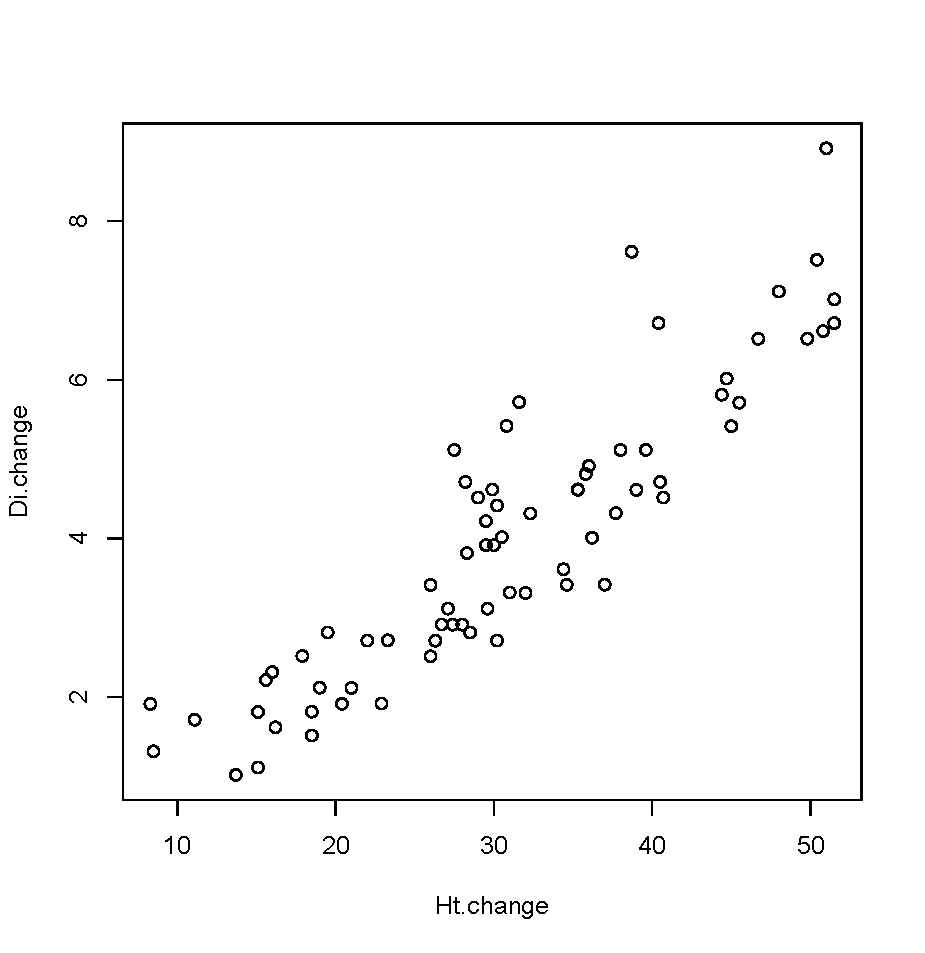
\includegraphics[width=0.4\textwidth]{6e.pdf}
\end{figure}
The diameter changes roughly increase with the height changes.

\setsection{8}
\subsection{}
To find the median, we need a value $m$ such that, for $a=1/2$:
\begin{align*}
a	& = \intg{-\infty}{m}{f(x)}{x}	\\
	& = \intg{0}{m}{\lambda  e^{-\lambda  x}}{x} \\
	& = 1-e^{-\lambda m}\\
\implies e^{-\lambda m} &= 1-a \\
\implies -\lambda m		&= \log (1-a) \\
\implies m				&= \lambda^{-1}\log\frac{1}{1-a} \\
&= \lambda^{-1}\log 2
\end{align*}

Similarly, for first and third quartiles, we use $a=1/4$, and $a=3/4$, respectively:\begin{align*}
Q_1=\lambda^{-1}\log\frac{1}{1-\frac{1}{4}}=\lambda^{-1}\log\frac{4}{3}\\
Q_3=\lambda^{-1}\log\frac{1}{1-\frac{3}{4}}=\lambda^{-1}\log 4
\end{align*}

\subsection{}
As with the previous problem:\begin{align*}
a	& = \intg{-\infty}{m}{f(x)}{x}	\\
	&= \intg{1}{m}{\frac{\alpha }{x^{\alpha +1}}}{x} \\
	&= 1-m^{-\alpha}\\
\implies m &= \sqrt[\alpha]{\frac{1}{1-a}}\\
&= \sqrt[\alpha]{2} \\
Q_1 &= \sqrt[\alpha]{\frac{4}{3}}\\
Q_3 &= \sqrt[\alpha]{4}
\end{align*}

\setsection{13}
The pmf is $f(x)=\binom{20}{x}0.3^x0.7^{20-x}$. So, the cdf $F(x)=\sum_{i=0}^xf(i)$. Then, there is no such $q$, since 2 is too small ($F(2)<0.04$) and 3 is too large ($F(3)>0.1$).

\setsection{14}
\subsection{}
One the QQ plot, the points showed a close fit to the straight line, but the histogram was never symmetric, only sometimes unimodal, and rarely mound-shaped.
\subsection{}
While the quality of the fit stayed good, the histograms only had a marginal improvement in terms of resembling a normal distribution (symmetric, unimodal and mound-shaped).
\subsection{}
It seems that QQ-normal plots are better for visually determining whether or not data is normally distributed.

\setsection{15}
% Booktabs require to add \usepackage{booktabs} to your document preamble
\begin{table}[h]
\centering
\begin{tabular}{@{}rrrr@{}}
\toprule
x  & f & cf & cdf=cf/total \\ \midrule
4  & 1 & 1  & 0.1          \\
7  & 1 & 2  & 0.2          \\
8  & 1 & 3  & 0.3          \\
9  & 2 & 5  & 0.5          \\
13 & 1 & 6  & 0.6          \\
18 & 3 & 9  & 0.9          \\
21 & 1 & 10 & 1.0          \\ \bottomrule
\end{tabular}
\end{table}
\begin{figure}[!ht]
\centering
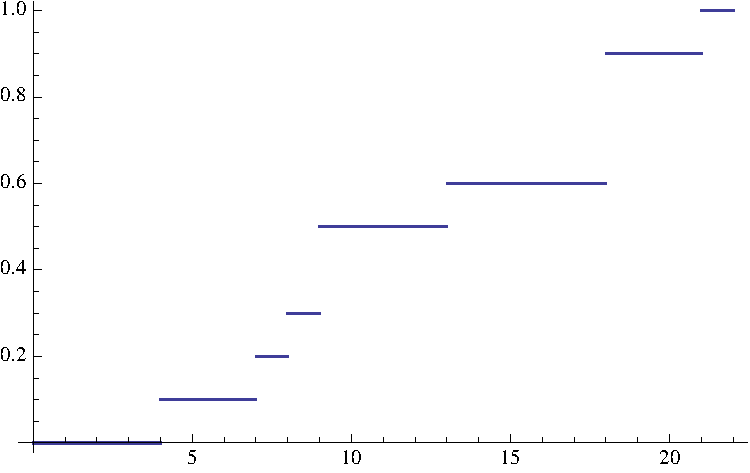
\includegraphics[width=0.4\textwidth]{15b.pdf}
\end{figure}

\newpage

\setsection{17}
\begin{figure}[!ht]
\centering
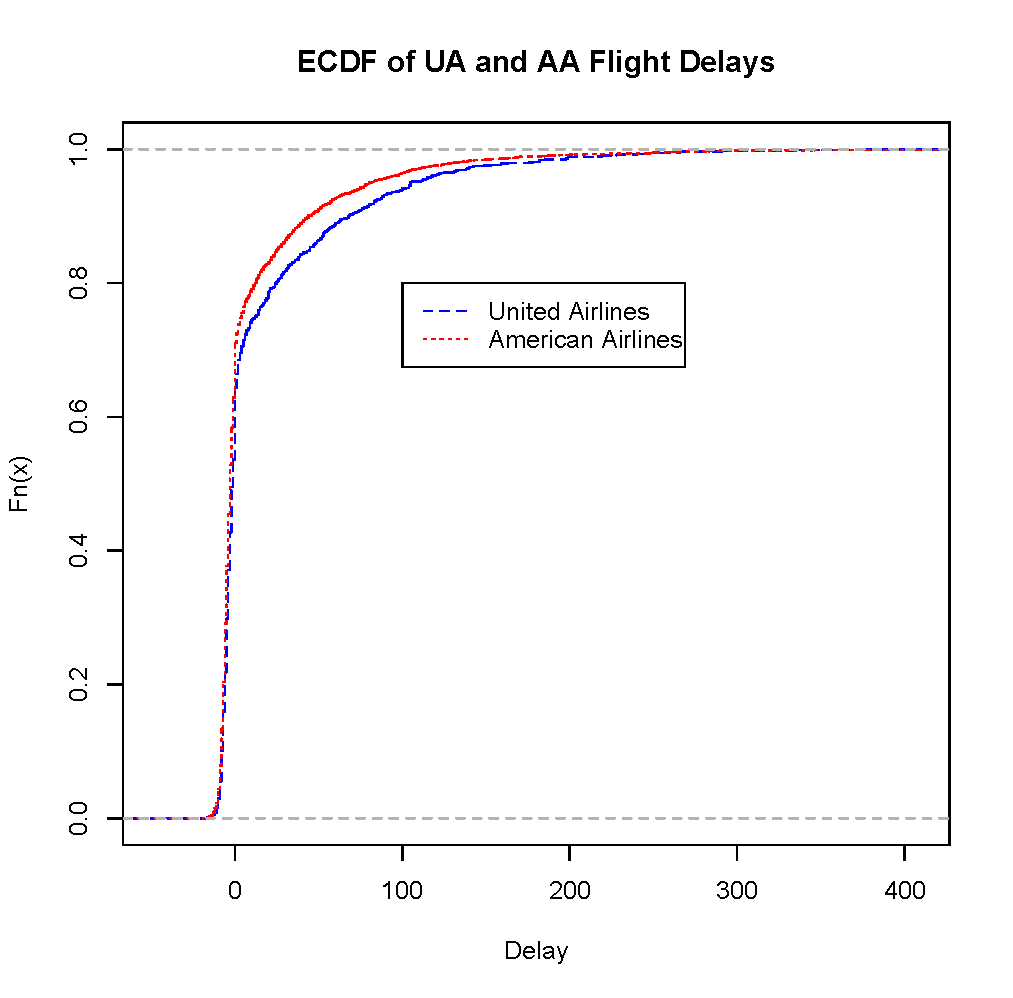
\includegraphics[width=0.4\textwidth]{17.pdf}
\end{figure}

From the plot, we can see that for a small range of delay times, the ecdf is higher for AA than for UA.

\end{document}
